\documentclass[a4paper, 11pt]{article}

% \usepackage[utf8]{inputenc}
\usepackage[T1]{fontenc}
\usepackage[brazilian]{babel}

\usepackage{nameref}
\usepackage{url}
\usepackage[hidelinks]{hyperref}
\hypersetup{
    pdftitle  = {Hotmart yt-dlp},
    % pdfauthor = {Tiago de Paula},
    % % bookmarks   = true,
    % pdfpagemode = UseOutlines,
    % %% Cores de Links %%
    colorlinks = true,
    linkcolor  = blue!30!black,
    urlcolor   = red!30!black,
    citecolor  = blue!30!black,
}

\usepackage[
    a4paper,
    headheight = 20pt,
    margin = 1in,
    top = \dimexpr 1in - 10pt \relax,
    bottom = \dimexpr 1in - 20pt \relax,
    footskip = 0pt,
  ]{geometry}
  \addtolength{\footskip}{20pt}
\usepackage{graphicx}
\usepackage{xcolor}
\usepackage{array}
\usepackage{booktabs}
\usepackage{multirow}
\usepackage{trimspaces}
\usepackage{xstring}
\usepackage[section]{placeins}
\usepackage{caption}
\usepackage{subcaption}
\usepackage{enumitem}
\usepackage{pgf}
\usepackage{tikz}
\usepackage{minted}

\usepackage{physics}
\usepackage{amsmath, amssymb, bm, mathtools}
\usepackage{etoolbox, xpatch, xspace}
% \usepackage[mathcal]{euscript}
% \usepackage[scr]{rsfso}
\usepackage{mathptmx, relsize, centernot}
% \usepackage{newtxtext, newtxmath}


\makeatletter

%% Símbolo QED %%
\newcommand{\qedsymbol}{\ensuremath{\mathsmaller\blacksquare}}

%% Marcadores de Prova: \direto, \inverso %%
\newcommand{\direto}[1][~]{\ensuremath{(\rightarrow)}#1\xspace}
\newcommand{\inverso}[1][~]{\ensuremath{(\leftarrow)}#1\xspace}

\undef\sum
%% Somatório: \sum_i^j, \bigsum_i^j %%
\DeclareSymbolFont{cmex10}{OMX}{cmex}{m}{n}
\DeclareMathSymbol{\sum@d}{\mathop}{cmex10}{"58}
\DeclareMathSymbol{\sum@t}{\mathop}{cmex10}{"50}
\DeclareMathOperator*{\sum}{\mathchoice{\sum@d}{\sum@t}{\sum@t}{\sum@t}}
\DeclareMathOperator*{\bigsum}{\mathlarger{\mathlarger{\sum@d}}}

%% Operadores de Conjunto: \pow(S), \Dom(S), \Img(S) %%
\DeclareSymbolFont{boondox}{U}{BOONDOX-cal}{m}{n}
\DeclareMathSymbol{\pow}{\mathalpha}{boondox}{"50}
\DeclareMathOperator{\Dom}{Dom}
\DeclareMathOperator{\Img}{Im}

\undef\Phi
%% Variantes gregas %%
\DeclareSymbolFont{cmr10}{OT1}{cmr}{m}{n}
\DeclareSymbolFont{cmmi10}{OML}{cmm}{m}{it}
\DeclareMathSymbol{\Phi}{\mathalpha}{cmr10}{"08}
\DeclareMathSymbol{\varpsi}{\mathalpha}{cmmi10}{"20}
\DeclareMathSymbol{\varomega}{\mathalpha}{cmmi10}{"21}

\undef\part
%% Família de Conjuntos ou Partição: \part{S} %%
\DeclareMathAlphabet{\part}{OMS}{cmsy}{m}{n}

\undef\natural
% Conjuntos Padrões: R, N, Z, C, Q %%
\undef\real
\DeclareMathOperator{\real}{\mathbb{R}}
\DeclareMathOperator{\natural}{\mathbb{N}}
\DeclareMathOperator{\integer}{\mathbb{Z}}
\DeclareMathOperator{\complex}{\mathbb{C}}
\DeclareMathOperator{\rational}{\mathbb{Q}}

%% Definição de Conjuntos: \set{ _ \mid _ } %%
\newcommand{\set}[1]{%
    \begingroup%
        \def\mid{\;\middle|\;}%
        \left\{#1\right\}
    \endgroup%
}

%% Novos Operadores: \modulo, \symdif, \grau %%
\DeclareMathOperator{\modulo}{~mod~}
\DeclareMathOperator{\symdif}{\mathrel{\triangle}}
\DeclareMathOperator{\grau}{deg}
\DeclareMathOperator{\mdc}{mdc}
\DeclareMathOperator{\sign}{sign}
\DeclareMathOperator{\signs}{sign*}

%% Operadores Delimitados: \abs{\sum_i^j}, x \equiv y \emod{n} %%
% \newcommand{\abs}[1]{{\left\lvert\,#1\,\right\rvert}}
\newcommand{\emod}[1]{\ \left(\mathrm{mod}\ #1\right)}

%% Vérices e Arestas %%
\DeclareMathOperator{\Adj}{Adj}
\DeclareMathOperator{\dist}{dist}

\makeatother

\usepackage{letltxmacro}
\usepackage{enumitem, amsmath, amsthm}
\usepackage[open]{bookmark}

\makeatletter

% problemas com o ambiente 'proof' do thmbox
\LetLtxMacro\ams@proof\proof
\LetLtxMacro\ams@end@proof\endproof

\usepackage[nocut,nothm]{thmbox}
\usepackage{thmtools}

% \AtBeginDocument{%
%     \LetLtxMacro\proof\ams@proof
%     \LetLtxMacro\endproof\ams@end@proof
% }

% Marcador lateral para teoremas
\newcommand*{\theorembookmark}{%
    \bookmark[
        dest = \@currentHref,
        rellevel = 1,
        keeplevel,
    ]{%
        \thmt@thmname\space\csname the\thmt@envname\endcsname
    }%
}


%% Ajusta espaços para o Display Mode %%
\newcommand{\reducemathskip}[1][0.5em]{%
    \setlength{\abovedisplayskip}{#1}%
    \setlength{\belowdisplayskip}{#1}%
    % \setlength{\abovedisplayshortskip}{#1}%
    % \setlength{\belowdisplayshortskip}{#1}%
}

%% Ambiente para Teoremas %%
\declaretheoremstyle[
    thmbox = M,
    preheadhook = \vskip1.5em,
    postheadhook = \theorembookmark\reducemathskip,
]{teorema}

\declaretheorem{theorem}[
    name = Teorema,
    % refname = {teorema,teoremas},
    % Refname= {Teorema,Teoremas},
    style = teorema,
]
\declaretheorem{lemma}[
    name  = Lema,
    style = teorema,
]
\declaretheorem{proposition}[
    name  = Proposição,
    style = teorema,
]
\declaretheorem{corollary}[
    name  = Corolário,
    style = teorema,
]

%% Ambiente para Definições %%
\declaretheorem{definition}[
    name = Definição,
    refname = {definição,definições},
    Refname= {Definição,Definições},
    %
    style = teorema,
    postheadhook = \theorembookmark\reducemathskip,
]
% Sem numeração
\declaretheorem{definition*}[
    name = Definição,
    refname = {definição,definições},
    Refname= {Definição,Definições},
    %
    style = definition,
    numbered = no,
    postheadhook = \reducemathskip
]

%% Lista de Casos %%
\newlist{casos}{enumerate}{2}
\setlist[casos]{
    wide,
    labelwidth    = {\parindent},
    listparindent = {\parindent},
    parsep        = {\parskip},
    topsep        = {0pt},
    label         = {\textbf{Caso \arabic*}:}
}
% \setlist[casos,2]{label=\textbf{Caso \arabic{casosi}\alph*}:}

%% Casos Nomeados: \item[Caso Base:] %%
\newlist{ncasos}{description}{2}
\setlist[ncasos]{
    wide,
    listparindent = {\parindent},
    parsep        = {\parskip},
    topsep        = {0pt}
}

\makeatother

\usepackage{silence}
\WarningFilter{mathptmx}{There are no bold math fonts}

\usepackage{mathpazo}
\usepackage[mathpazo]{flexisym}
\usepackage{breqn}

\DeclareMathOperator{\EX}{\mathbb{E}}
\newcommand*\Eval[3]{\left.#1\right\rvert_{#2}^{#3}}

\begin{document}
    \section{Instalação}

    Para instalar o \href{https://github.com/yt-dlp/yt-dlp}{\texttt{yt-dlp}} no Windows 11, abra o \href{https://learn.microsoft.com/en-us/windows/terminal/}{Terminal} no modo \href{https://learn.microsoft.com/en-us/powershell/}{PowerShell} e execute:

    \begin{minted}{powershell}
        winget install -e --id yt-dlp.yt-dlp
    \end{minted}

    \begin{center}
        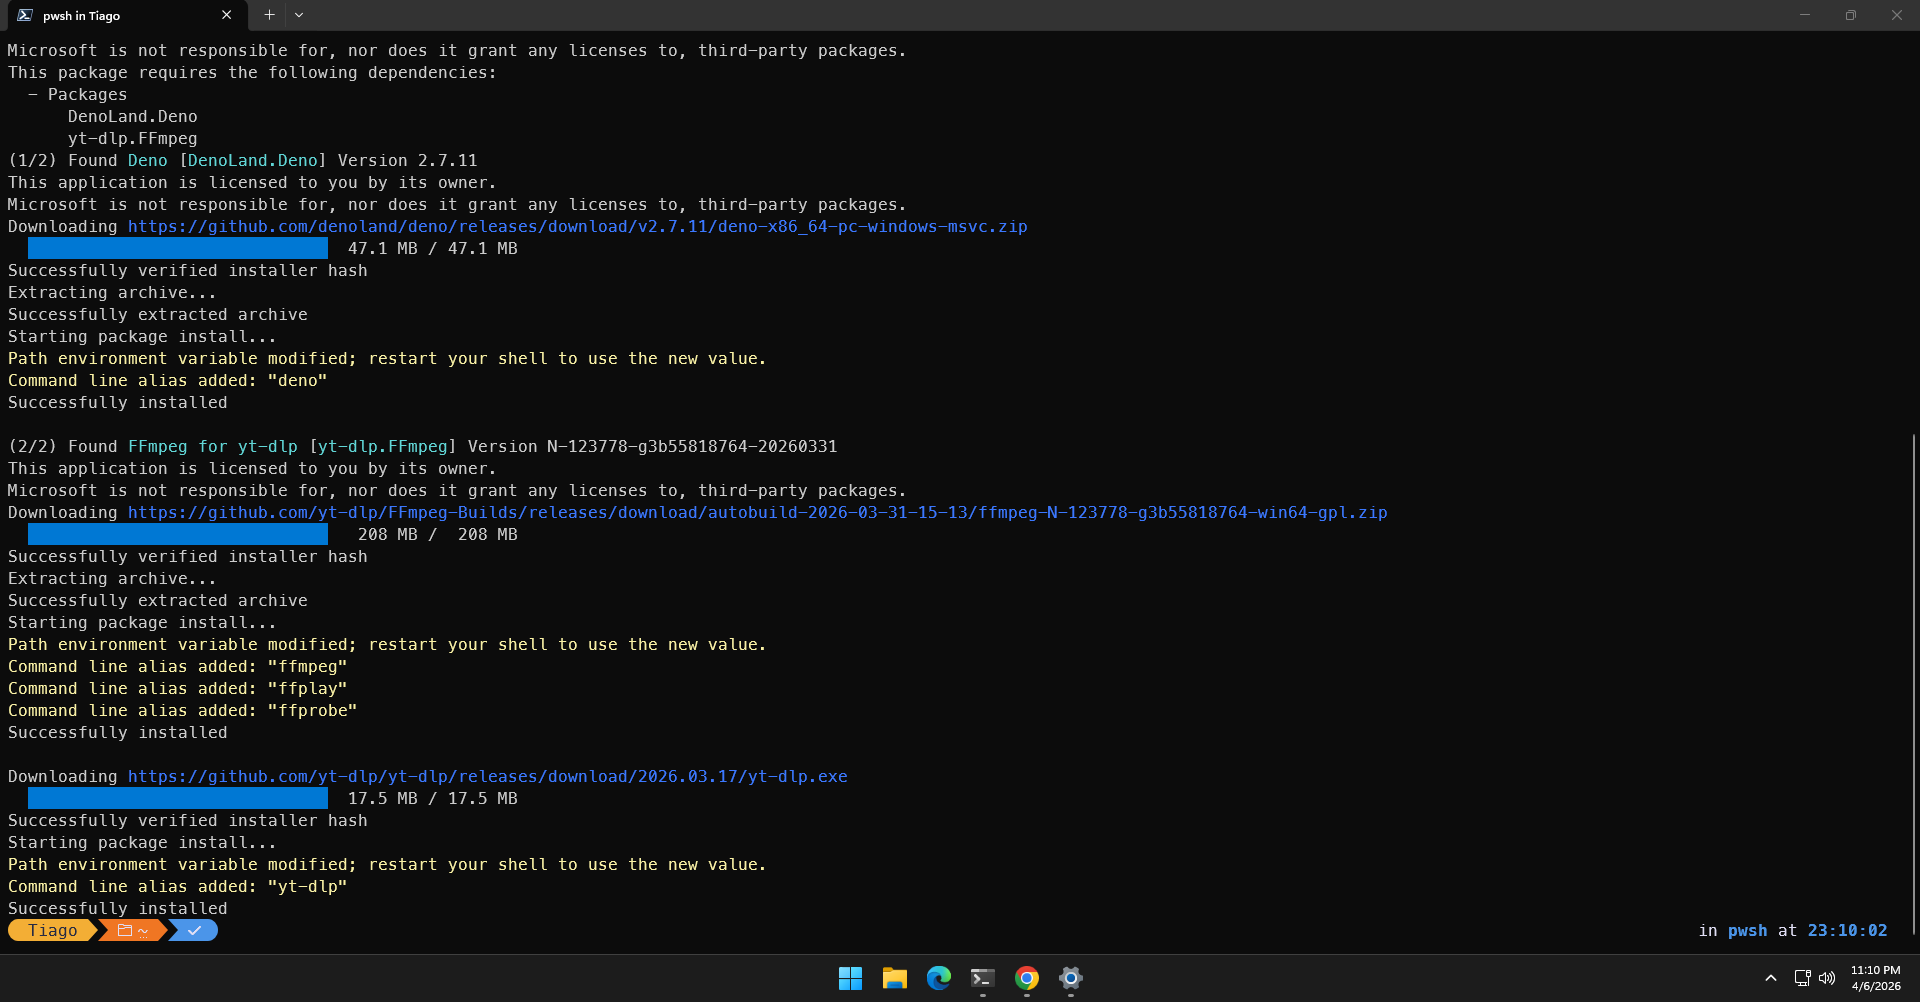
\includegraphics[width=0.75\textwidth]{figures/01.png}
    \end{center}

    \section{Download}

    Abra o vídeo desejado no \href{https://www.google.com.br/chrome/}{Google Chrome}, em seguida abra o \href{https://developer.chrome.com/docs/devtools}{Chrome DevTools} (\texttt{F12}) na aba \textit{Network} e pesquise por \texttt{m3u8}. Recarregue a página, espere o vídeo começar a carregar e copie a URL do arquivo \texttt{master-pkg-t-NNNNNNNNNNNNN.m3u8}, que será provavelmente o primeiro item da lista.

    \begin{center}
        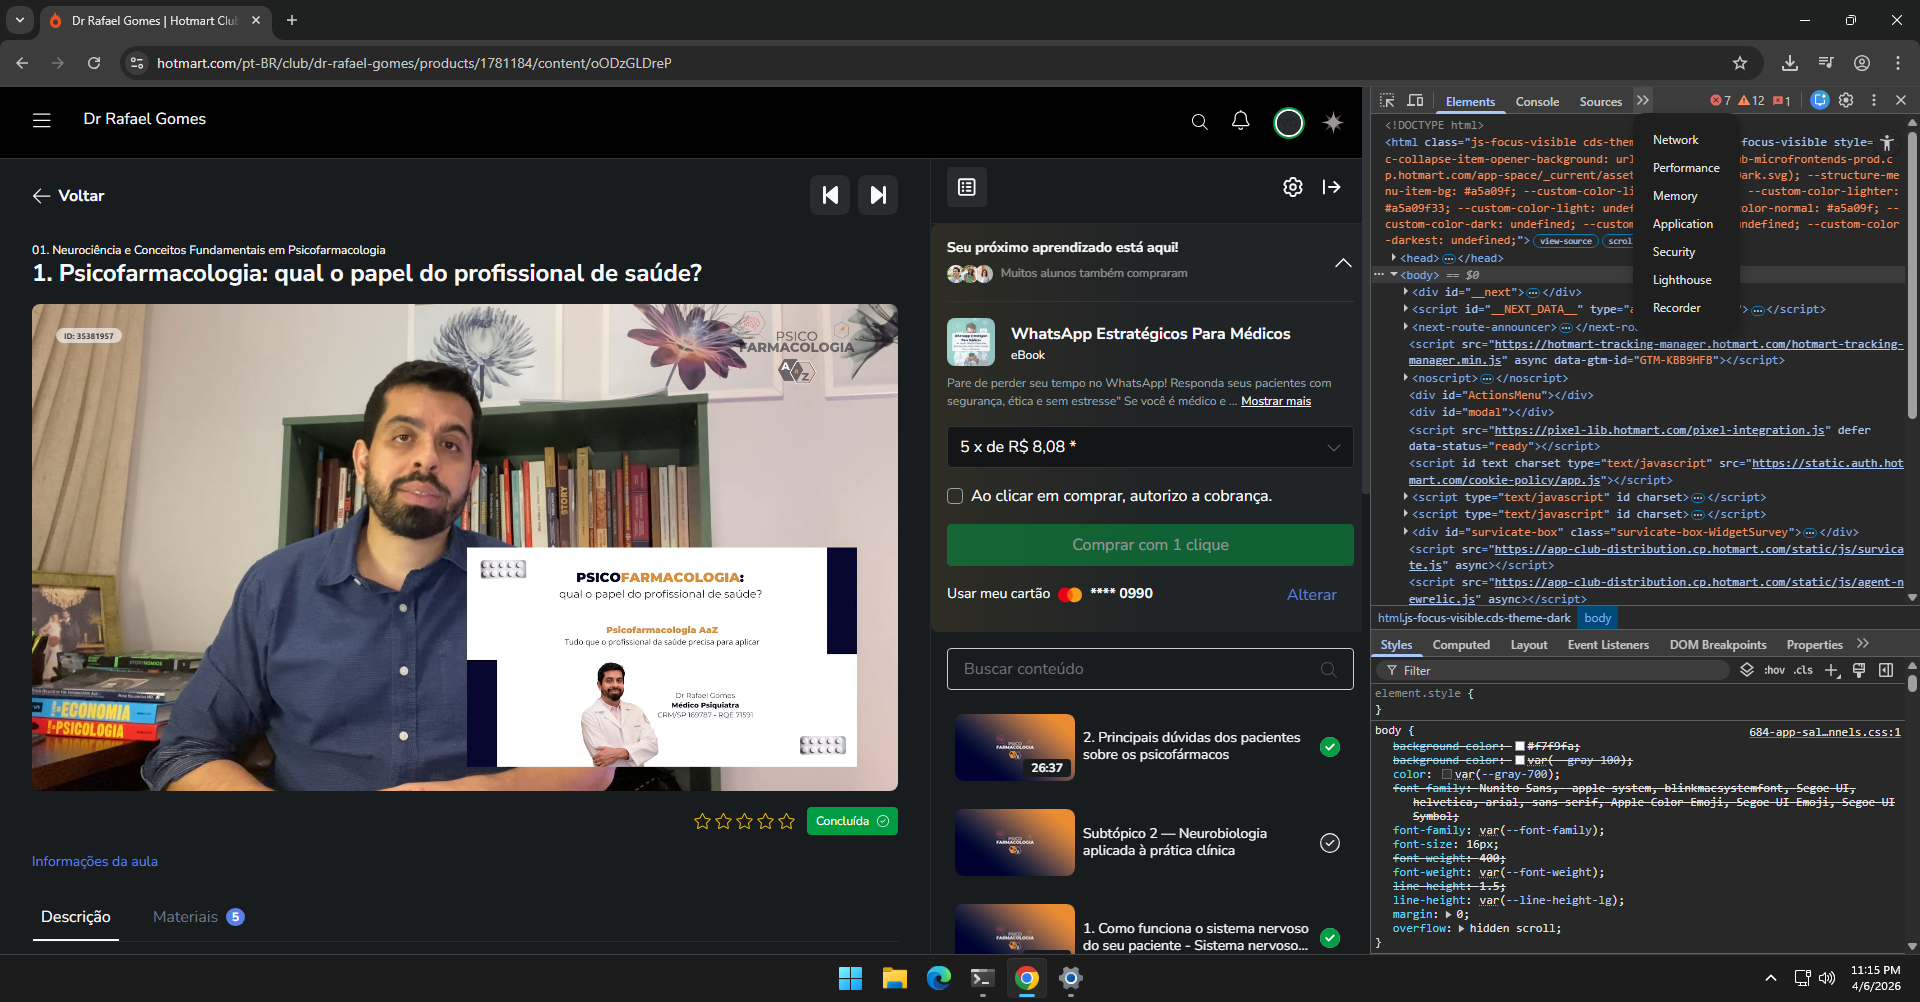
\includegraphics[width=0.75\textwidth]{figures/02.png}
    \end{center}

    \begin{center}
        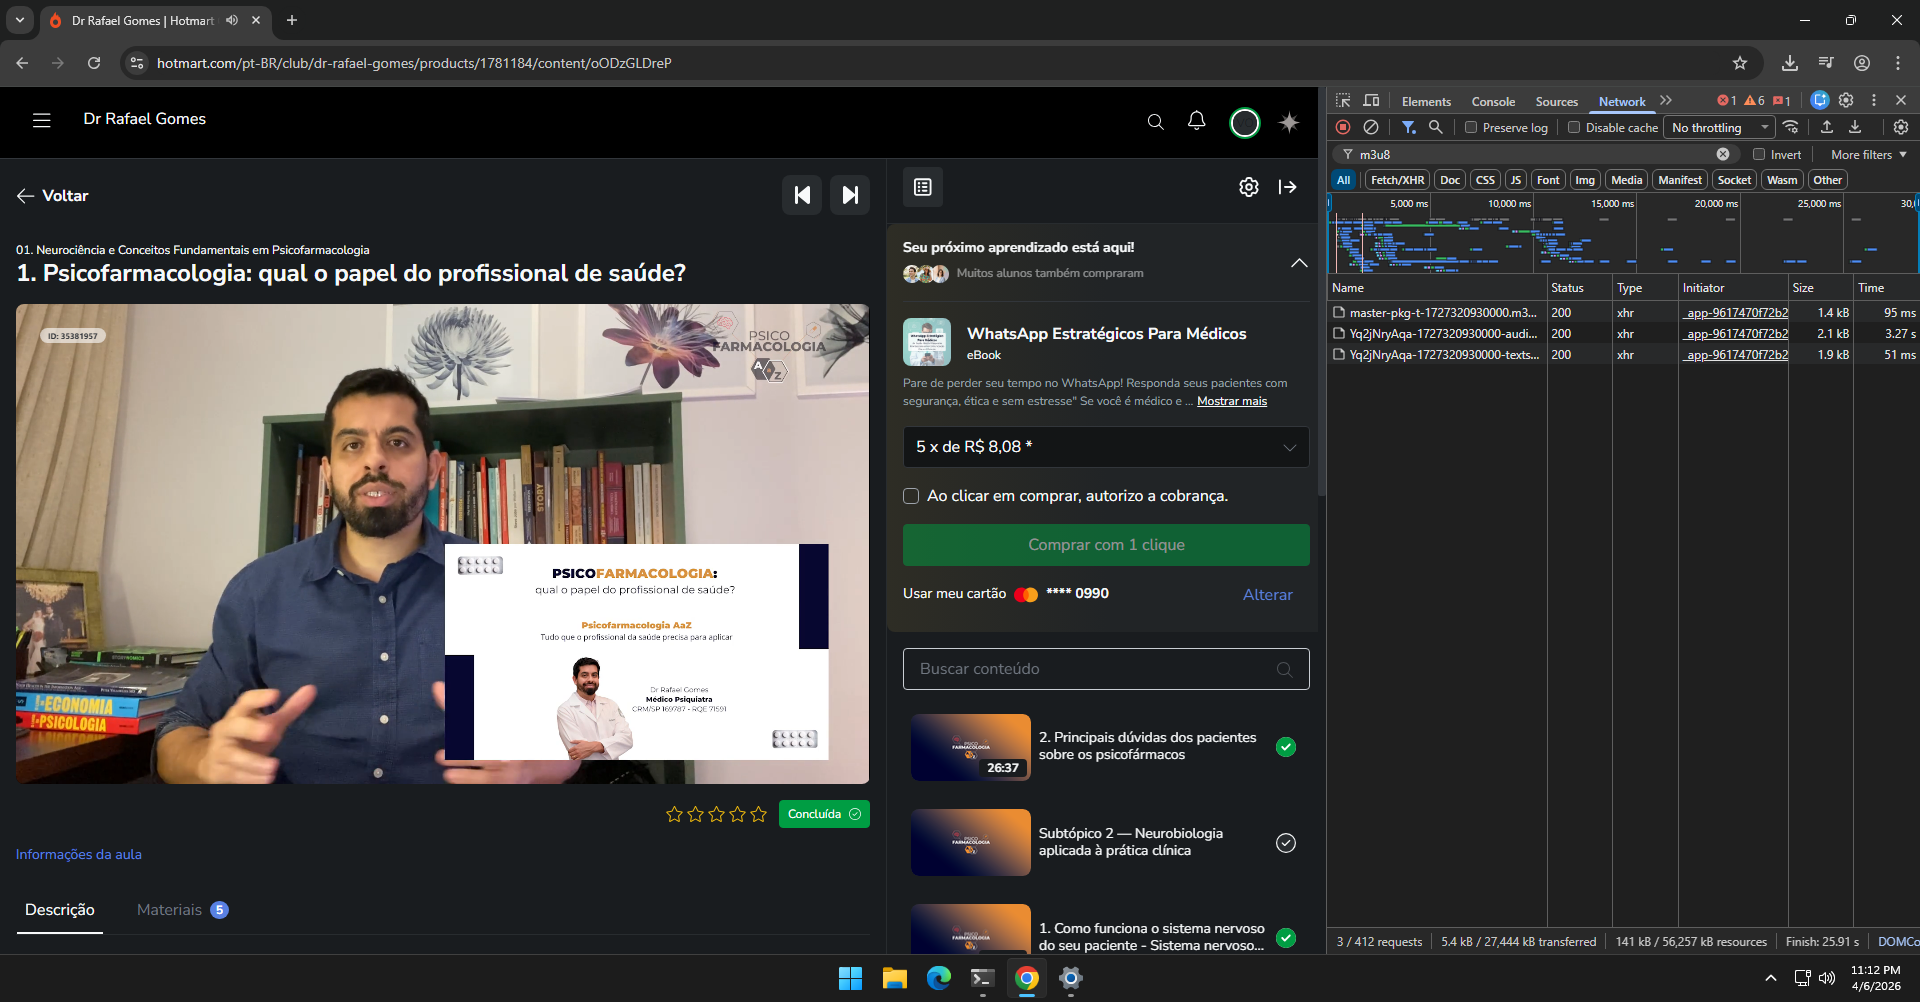
\includegraphics[width=0.75\textwidth]{figures/03.png}
    \end{center}

    \begin{center}
        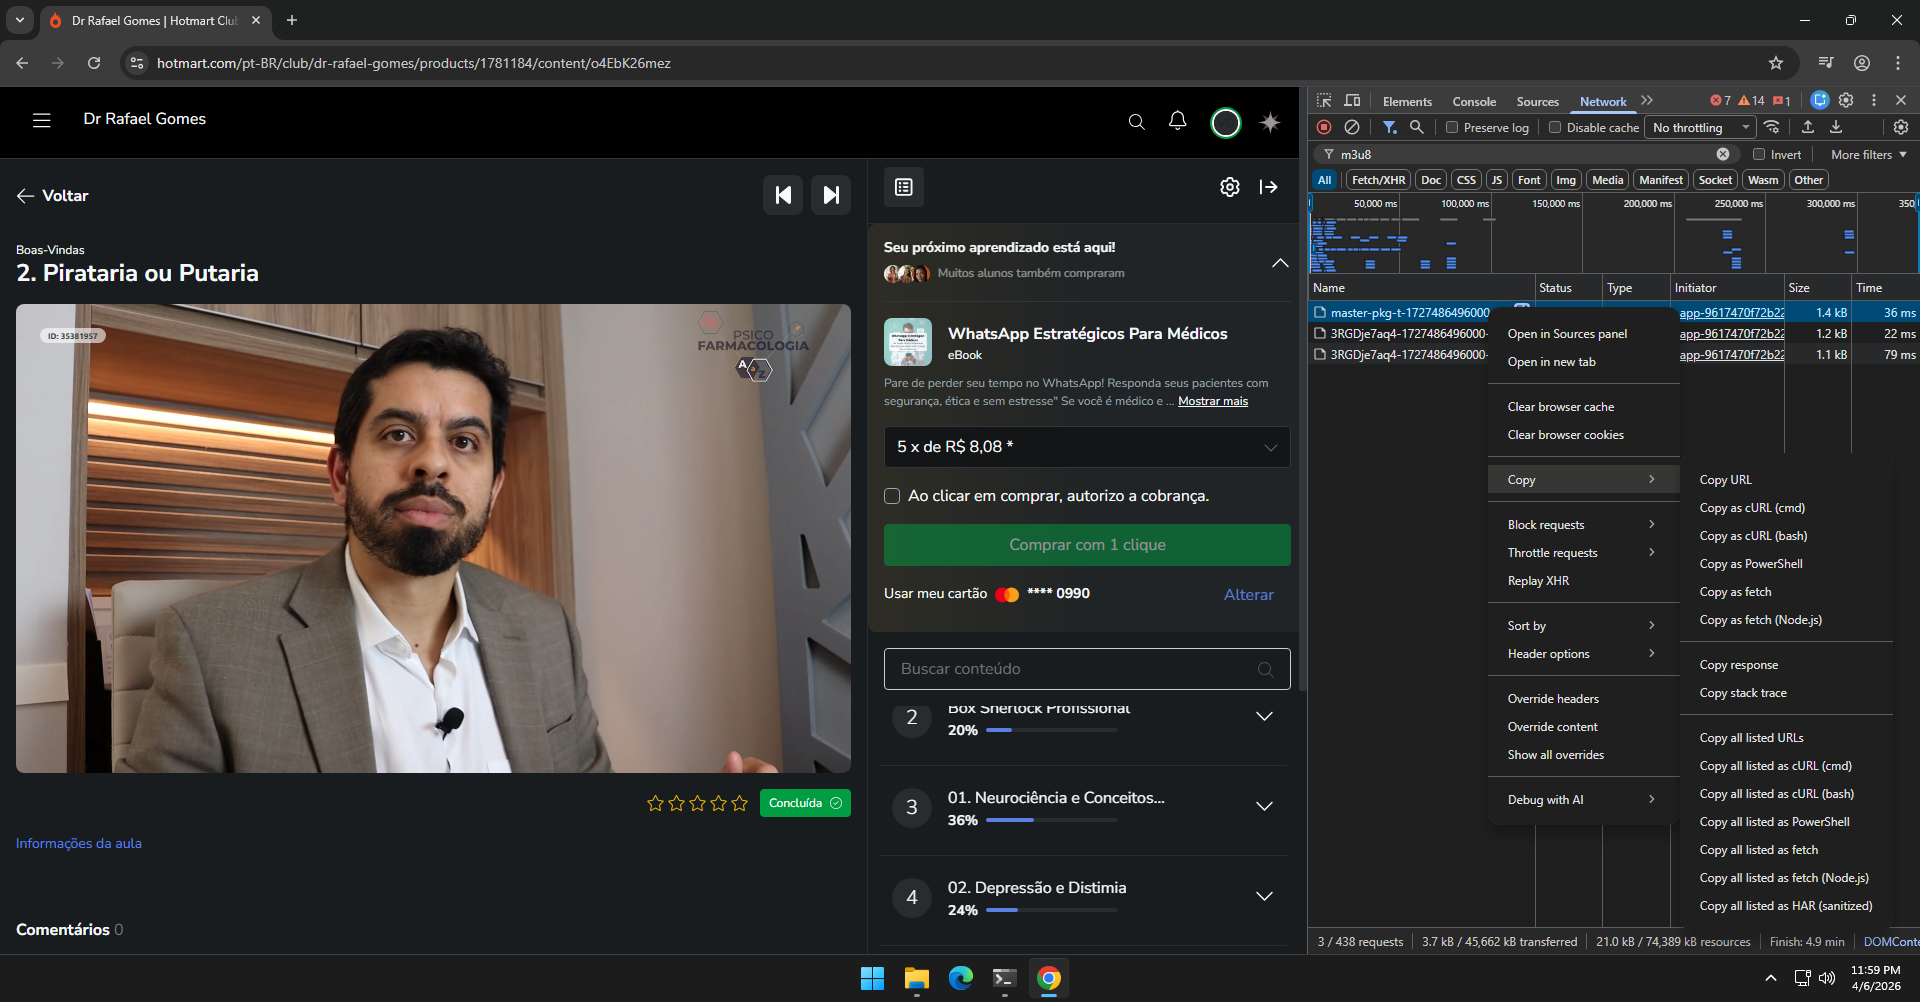
\includegraphics[width=0.75\textwidth]{figures/04.png}
    \end{center}

    Por fim, abra o Terminal no modo PowerShell novamente e digite o seguinte, trocando \mintinline{bash}{%URL%} pela URL copiada do Chrome DevTools:

    \begin{minted}[breaklines]{bash}
        yt-dlp -f bestvideo+bestaudio/best --concurrent-fragments 2 --referer https://player.hotmart.com '%URL%'
    \end{minted}

    \begin{center}
        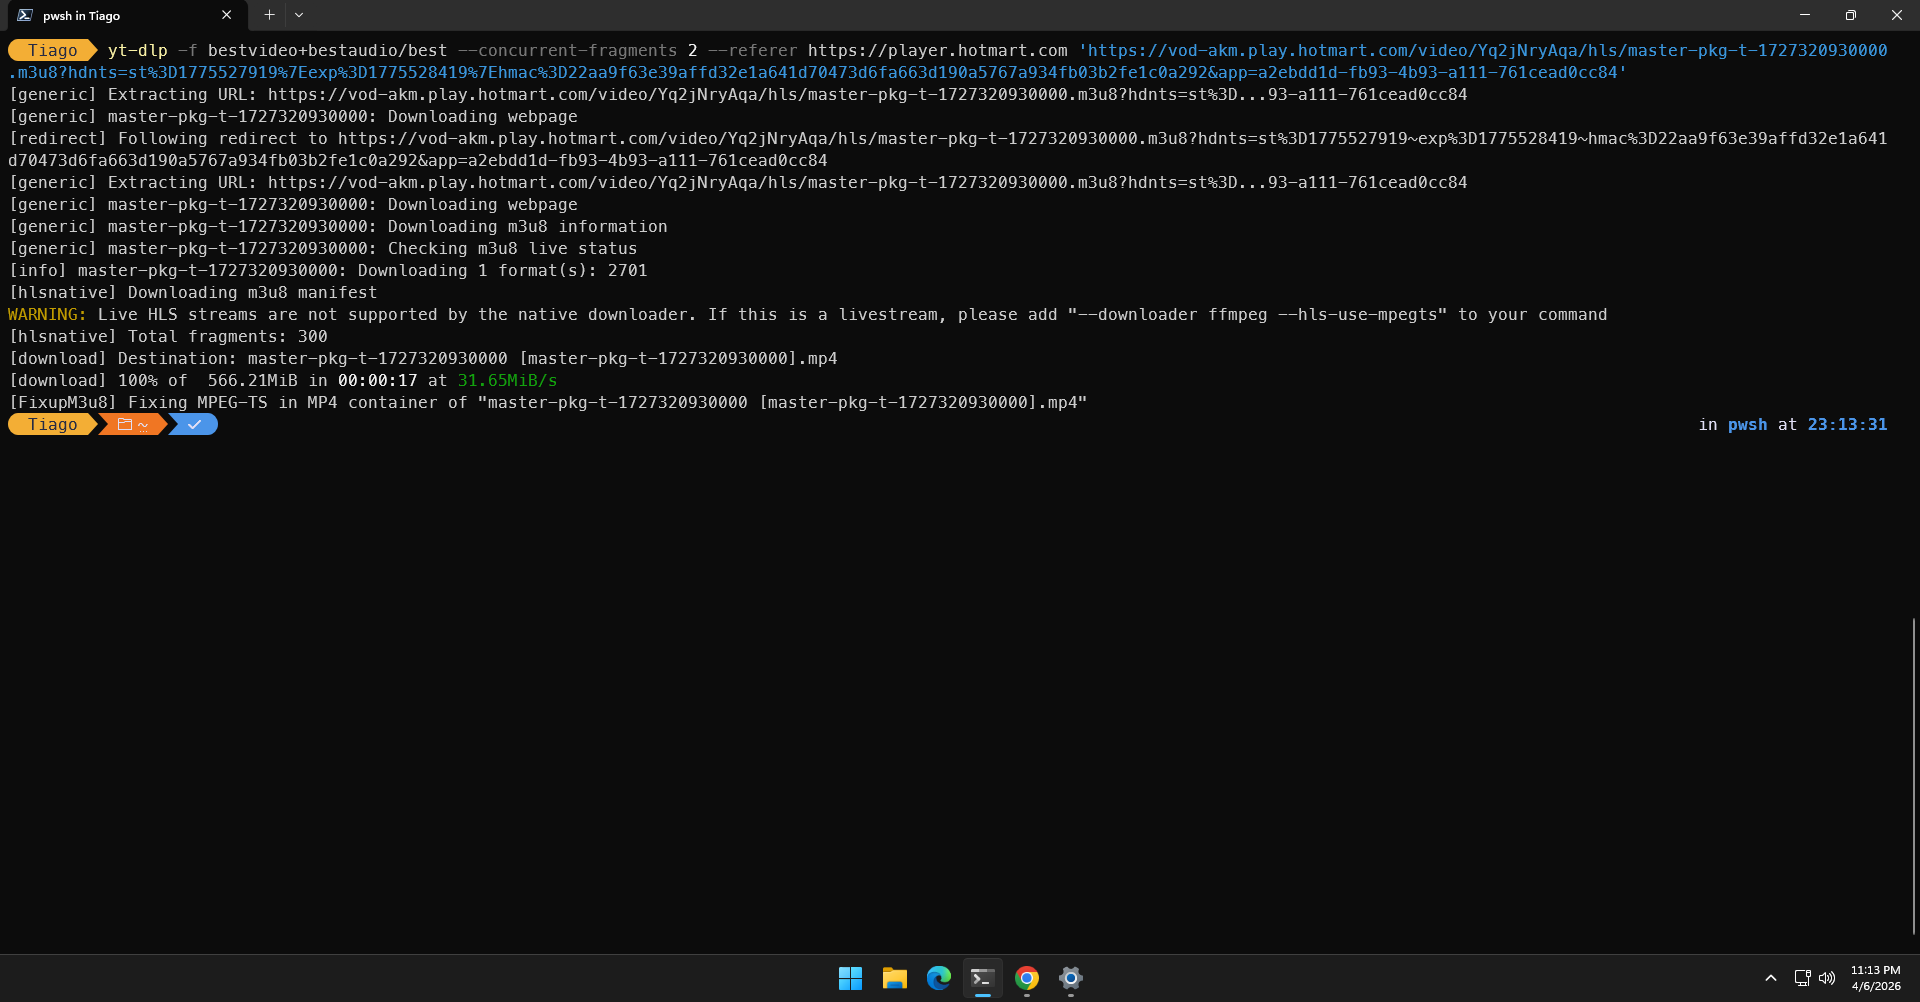
\includegraphics[width=0.75\textwidth]{figures/05.png}
    \end{center}
\end{document}
